\documentclass{assignment}
\UsingEnglish
\ProjectInfos*{Intro to Communication System}{EE140}{Fall, 2020}{Assignment 6}{Due time : 10:15, Oct 30, 2020 (Friday)}{陈稼霖}{45875852}
\begin{document}
\begin{prob}[Noise in DSB-SC Receiver, 30pts]
    A DSB-SC modulated signal in transmitted over a noisy channel. The power spectral density of the noise is shown in Figure \ref{A-6-P-1}. The message bandwidth is $3$ kHz and the carrier frequency is $200$ kHz. Assuming that the average power of the modulated signal is $12$ watts, determine the input signal-to-noise ratio (predetection SNR), output signal-to-noise ratio (postdetection SNR) and the detection gain (input SNR / output SNR).
    \begin{figure}[h]
        \centering
        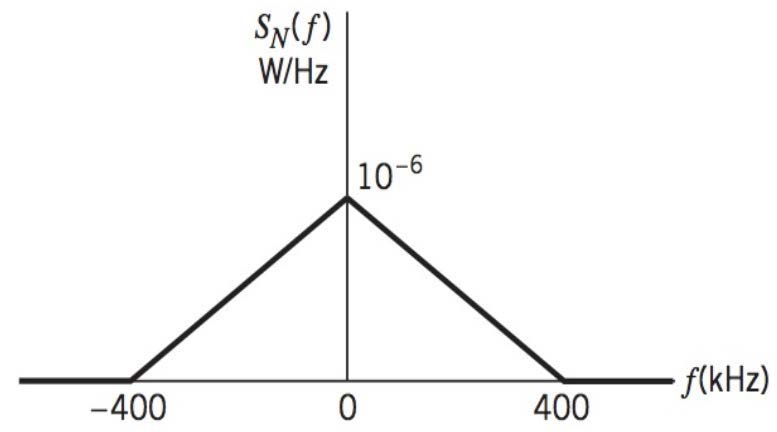
\includegraphics[width=.5\columnwidth]{A-6-P-1.jpg}
        \caption{}
        \label{A-6-P-1}
    \end{figure}
\end{prob}
\begin{sol}

\end{sol}

\begin{prob}[Noise in SSB Receiver, 25pts]
    Derive the equation for $y_D(t)$ for an USB-SSB system assuming that the noise is expanded about the frequency $f_c+\frac{W}{2}$. Derive the output SNR (postdetection SNR), detection gain and the figure of merit. Determine and plot the power spectral density of the in-phase component $n_c(t)$ and the quadrature component $n_s(t)$ of the narrowband noise.
\end{prob}
\begin{sol}
    
\end{sol}

\begin{prob}
    Assume an AM system operates with a modulation index $a=0.4$. The message signal is $m(t)=5\cos(10\pi t)$.
    \begin{itemize}
        \item[1)] Compute the transmission efficiency.
        \item[2)] Assume the envelope detector operates above the threshold. Compute the output SNR (postdetection SNR) in decibel relative to the input SNR.
        \item[3)] Compute the output SNR in decibels relative to the baseband SNR ($P_T/N_0W$).
        \item[4)] Keep $P_T$ (the average power of modulated signal) unchanged, determine the improvement (in decibels) in the output SNR if the modulation index is increased from $0.4$ to $0.8$. (Hint: Since the input SNR and baseband SNR are unchanged, we can calculate the improvement of output SNR based on its relationship with the input SNR and baseband SNR.)
    \end{itemize}
\end{prob}
\begin{sol}
    \begin{itemize}
        \item[1)] 
        \item[2)] 
        \item[3)] 
        \item[4)] 
    \end{itemize}
\end{sol}

\begin{prob}[Noise in FM Receiver and FDM, 20pts]
    An FDM system uses single-sideband modulation to from the baseband, and FM modulation for transmission of the baseband. Assume that there are eight channels and that all eight message signal have equal power $P_0$ and equal bandwidth $W$. For each signal, only the upper sideband is transmitted. The sub-carrier waves used for the first stage of modulation are defined by $c_k(t)=A_k\cos(2\pi kf_0t),0\leq k\leq 7$. The width of the guardbands is $3$ W. The received signal consists of the transmitted FM signal plus white Gaussian noise of zero mean and two-sided power spectral density $N_0/2$. Assume the frequency discriminator at the receiver operates above the threshold.
    \begin{itemize}
        \item[1)] Sketch the power spectral density of the signal produced at the frequency discriminator output, showing both the signal and the noise components.
        \item[2)] Find the relationship between the subcarrier amplitudes $A_k$ such that the SSB modulated signals corresponding to different channels have equal output SNRs at the frequency discriminator output.
    \end{itemize}
\end{prob}
\begin{sol}
    \begin{itemize}
        \item[1)] 
        \item[2)] 
    \end{itemize}
\end{sol}
\end{document}